\documentclass{article}
\usepackage{graphicx}
\usepackage{geometry}
\usepackage[hidelinks]{hyperref}
% \usepackage{biblatex}

\geometry{
    a4paper,
    total={170mm,257mm},
    left=20mm,
    top=20mm,
}

% \bibliography{references}

\title{Single-actor bicycle crash classification guide}
\author{
  Benjam\'in Gonz\'alez\\
  \small{\href{mailto:b.gonzaleztoledo@tudelft.nl}{B.GonzalezToledo@tudelft.nl}}
  }
\date{\today}

\begin{document}

\maketitle

\begin{figure}
    \centering
    \includegraphics[angle=90, height = \textheight]{class-mindmap-v2.png}
    \caption{Flowchart of bicycle crash classification.}
    \label{fig: flowchart}
\end{figure}

\begin{figure}[h]
    \centering
    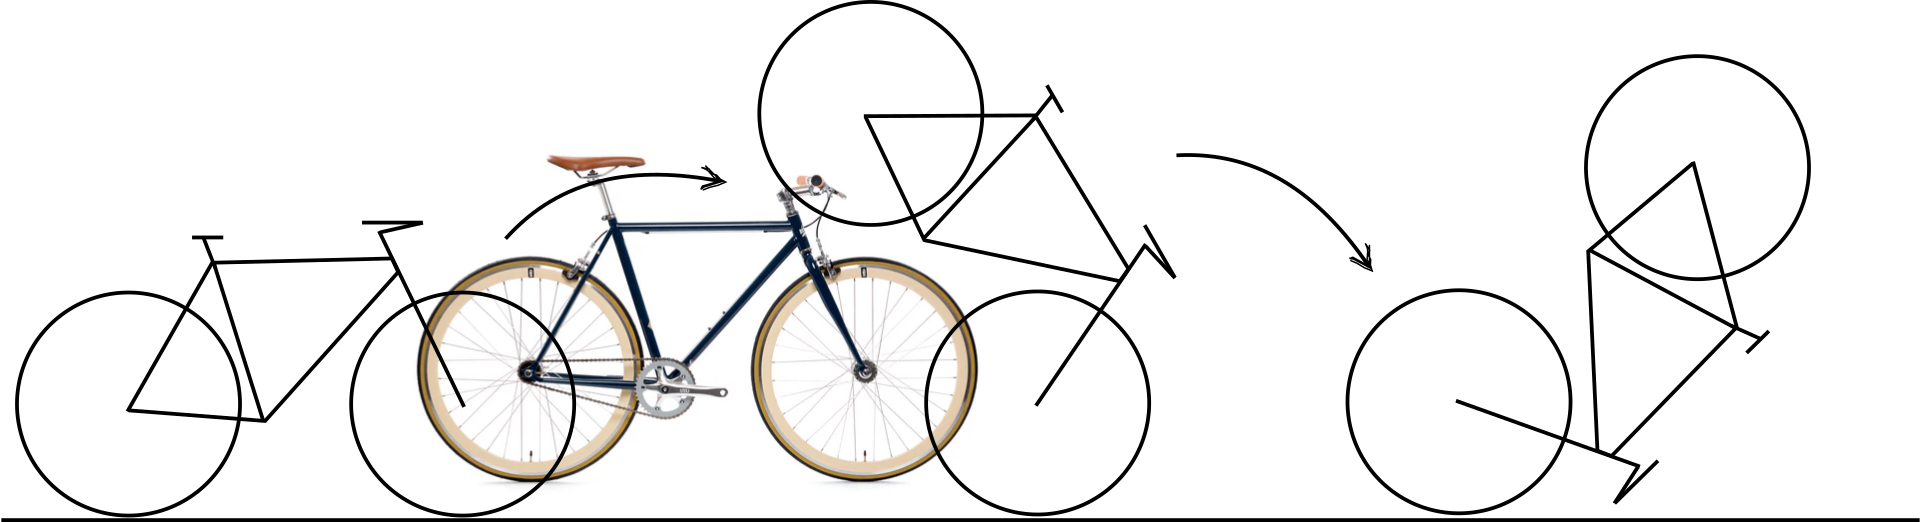
\includegraphics[width=\linewidth]{pitch-over.png}
    \caption{Simple diagram of pitch-over motion.}
    \label{fig: pitchover}
\end{figure}

\begin{figure}[h]
    \centering
    \includegraphics[width=\linewidth]{roll-over.png}
    \caption{Simple diagram of roll-over motion.}
    \label{fig: rollover}
\end{figure}
\section{Introduction}

This document aims to guide you to understand the proposed classification \cite{Jac04} of single-actor bicycle-crashes and label the samples sent to you.

\subsection{What is a Single-actor bicycle crash?}

A single-actor bicycle-crash is an event where the normal riding of the bicycle is disrupted and ends in a crash with no other road users involved.

\section{Bicycle dynamics-oriented classification}

The proposed workflow to classify the crash according to the observed characteristics is composed by three sub-categories: motion, interaction and mechanism (see Figure \ref{fig: flowchart}).

\subsection{Motion of the bicycle}

This is related to the main motion of the rear frame of the bicycle while the crash is occuring.
%
Due to the dynamics of the bicycle, and following the common simplification to its analysis, we find two main motions related to the degrees of freedom: pitch-over and roll-over.
%
Additionally, the roll-over motion includes its own sub-classification according to the direction of rotation with respect to the initial motion.
% 
Please visit \url{https://youtube.com/shorts/_etyqSpH10c?feature=shared} to watch an example of a crash where the final rotation is in the opposite direction of the initial motion.
%
This is particularly challenging to represent in a normal drawing so the visual explanation is on the make.

\begin{itemize}
    \item \textbf{Pitch-over (P):} The main characteristic of this motion is one of the wheels lifting from the ground and following a trajectory that finishes with the front wheel behind the rear wheel.
    \item \textbf{High-side (H):} Characterised for a sudden deceleration of the wheel while in lateral motion, which leads to a violent roll motion in the opposite direction of the initial motion.
    \item \textbf{Low-side (L):} The human-bicycle system follows an excessive roll motion in the same direction as at the beginning.
\end{itemize}

\section{Force}

For this research, the bicycle is assumed as an interface between the human and the environment.
%
Therefore, the bicycle is subjected to forces from the environment and also to forces created by the human.


\begin{itemize}
    \item \textbf{External forces (E):} Mechanical forces that result from the interaction of the human-bicycle system with the environment.
    \item \textbf{Rider forces (I):} This makes reference to the control inputs from the human to the vehicle.
\end{itemize}

\section{Mechanism of crash}

Here we detail mechanisms that made possible bicycle riding, however, in the analysis of crashes, we delve into the failure of these mechanisms.

\subsection{External mechanisms}
\begin{itemize}
    \item \textbf{Tyre forces (T):} Forces acting in the tyre-ground interface, principally grip and normal. The failure mechanism is the slide.
    \item \textbf{Aerodynamic forces (A):} Aerodynamic forces which are studied as a resultant in the centre of pressure of the system.
    \item \textbf{Body excerted forces (D):} All forces that interact with the human bicycle system as contact inputs, e.g. collisions.
\end{itemize}

\subsection{Rider mechanisms}
\begin{itemize}
    \item \textbf{Brake input (B):} To decrease the speed, the rider has control on the brakes, which input can be erroneous and go out of the boundaries of their capabilities of control, resulting in excessive load transfer.
    \item \textbf{Steering torque (S):} The main control input on the bicycle, this allows the rider to balance the bicycle as an inverted pendulum.
    \item \textbf{Power input (W):} Pedal force applird from the rider, this creates the forward motion of the bicycle.
        %
        The failure mechanism is excessive load transfer or sudden disengagement of the foot-pedal interface.
\end{itemize}

\subsection{Location}

We can identify the direction with respect to the reference frame of the bicycle where the force acts: longitudinal or lateral.
%
In line manner, it is possible to differenciate the region of the system where the main principal interaction occurs: front or rear.

\section{Force characteristics}


\begin{itemize}
    \item \textbf{Step:} A force that instantaneously changes from zero to a constant value and remains at that level indefinitely. It represents a sudden application of force.
    \item \textbf{Ramp:} A force that increases linearly with time, modeling a steadily growing input to a system.
    \item \textbf{Impulse:} A high-magnitude force applied over a very short duration.
    \item \textbf{Periodic:} A force that repeats at regular time intervals, such as sinusoidal.
\end{itemize}


\section{Example}

Let's do an example using the following video \url{https://youtube.com/shorts/VZibdrdhdgM?feature=shared}.

First, it is observed that the main motion of the bicycle in the crash is related to roll angle.
%
Additionally, it is in the same direction of the beginning of the motion.
%
Therefore, this corresponds to the category low-side (L).


Second, there are no visible wrong rider control inputs, which leads to a external force mechanism (E).
%
Additionally, it is not possible to determine if aerodynamics played a major role and there is no visible external body perturbation.
%
For this reason, we conclude that the fail mechanism occurs at the tyre-ground interface (T), being reasonable to assume that the event started in the front wheel (F).


Third, from tyre mechanics it is known that tyres have a saturation margin where available grip reaches a limit.
%
In this case, this force relation can be assumed as an step force, where the available grip suddenly decreases and it is not recovered.


Finally, the classification of this crash would be \textbf{LE-TF-Step}, front slide low side.

\begin{thebibliography}{9}

    \bibitem{Jac04} Elin K. Jacob (2004):  Classification and Categorization: A Difference that makes a Difference. Graduate School of Library and Information Science. University of Illinois at Urbana-Champaign. \url{http://hdl.handle.net/2142/1686}

\end{thebibliography}


\end{document}
